%!TEX options=--shell-escape
\documentclass[tikz]{standalone}
\usepackage[T1]{fontenc}
\usepackage[utf8]{inputenc}
\usepackage{xcolor}
\usepackage{amsmath}
\usepackage{amssymb}
\usepackage{hyperref}
\usepackage{accsupp}    
\usepackage{graphicx}
\usepackage{mathtools}
\usepackage{pagecolor}
\usepackage{amsmath} % for \dfrac
\usepackage{tikz}
\tikzset{>=latex} % for LaTeX arrow head
\usepackage{pgfplots} 
\usepackage[edges]{forest}
\usetikzlibrary{patterns, backgrounds, arrows.meta}
\setlength{\parindent}{0cm}
\setlength{\parskip}{1em}
\usepackage{braket}

\usetikzlibrary{patterns}
\def\rescale{0.142857}


% Figure 4.3 https://arxiv.org/pdf/1709.02318.pdf 

\begin{document}
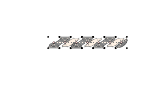
\begin{tikzpicture}[scale=\rescale]

 \foreach \x in {0, 2, 4}{
    \draw[line width = 0.25 * \rescale,black, opacity = 0.85, fill=gray](\x + 1,1) arc (0:180:-0.5) -- cycle;
    \draw[line width = 0.25 * \rescale,black, opacity = 0.85, fill=gray](\x,0) arc (180:0:0.5) -- cycle;
    } 
    \draw[line width = 0.25 * \rescale,black, opacity = 0.85,fill=gray](2,0) arc (180:0:0.5) -- cycle;

   \foreach \x in {0, 2, 4}{
       \fill[line width = 0.25 * \rescale,draw=black, opacity = 0.85,fill=gray, rounded corners= \rescale *3pt] (\x + 0.15, 0.15) -- (\x + 1.15, 0.85) -- (\x+1.85, 0.85) -- (\x+0.85, 0.15)  -- cycle;
        }

    \foreach \x in {1, 3, 5}{
   \fill[line width = 0.25 * \rescale,draw=black, fill=yellow!40!red!10, opacity = 0.85,rounded corners= \rescale *3pt] (\x + 0.15, 0.15) -- (\x + 1.15, 0.85) -- (\x+1.85, 0.85) -- (\x+0.85, 0.15)  -- cycle;
    }


    % Horizontal Lines
    \foreach \x in {0, 2, 4}{
    \draw[line width = \rescale, dash pattern={on 0.5pt off 0.5pt on 0.5pt off 0.5pt}, yellow!40!red!10] (\x + 0.5, 0.5) to (\x + 1.5, 0.5);
    } 

    \foreach \x in {0, 2, 4}{
    \draw[line width = \rescale, dash pattern={on 0.5pt off 0.5pt on 0.5pt off 0.5pt}, gray] (\x + 1.5, 0.5) to (\x + 2.5, 0.5);
   }

    \foreach \x in {1, 3, 5}{
        \draw[line width =  \rescale, dash pattern={on 0.5pt off 0.5pt on 0.5pt off 0.5pt}, gray] (\x, 0) to [bend right=45](\x+0.5, 0.5);
        \draw[line width =  \rescale, dash pattern={on 0.5pt off 0.5pt on 0.5pt off 0.5pt}, gray] (\x + 1, 0) to [bend left=45](\x+0.5, 0.5);

        \draw[line width = \rescale, dash pattern={on 0.5pt off 0.5pt on 0.5pt off 0.5pt}, yellow!40!red!10] (\x, 1) to [bend left=45](\x+0.5, 0.5);
        \draw[line width = \rescale, dash pattern={on 0.5pt off 0.5pt on 0.5pt off 0.5pt}, yellow!40!red!10] (\x + 1, 1) to [bend right=45](\x+0.5, 0.5);

    }

    \foreach \x in {0, 2, 4}{
        \draw[line width = \rescale, dash pattern={on 0.5pt off 0.5pt on 0.5pt off 0.5pt}, yellow!40!red!10] (\x, 0) to [bend right=45](\x+0.5, 0.5);
        \draw[line width = \rescale, dash pattern={on 0.5pt off 0.5pt on 0.5pt off 0.5pt}, yellow!40!red!10] (\x + 1, 0) to [bend left=45](\x+0.5, 0.5);

        \draw[line width = \rescale, dash pattern={on 0.5pt off 0.5pt on 0.5pt off 0.5pt}, gray] (\x + 2, 1) to [bend left=45](\x+2.5, 0.5);
        \draw[line width = \rescale, dash pattern={on 0.5pt off 0.5pt on 0.5pt off 0.5pt}, gray] (\x + 3, 1) to [bend right=45](\x+2.5, 0.5);

    }

    % Endcap
    \filldraw[line width =0.25*\rescale, fill=gray] (6, 0.15) -- (7, 0.85) to [bend left=85] (6, 0.15);
    \draw[line width = \rescale, dash pattern={on 0.5pt off 0.5pt on 0.5pt off 0.5pt}, yellow!40!red!10] (6, 0) to[bend right=45] (6.5, 0.5);
    \draw[line width = \rescale, dash pattern={on 0.5pt off 0.5pt on 0.5pt off 0.5pt}, yellow!40!red!10] (7, 1) to[bend left=45] (6.5, 0.5);


    \foreach \x in {0, 1,..., 6}{
           \filldraw[line width = 0.25 * \rescale,draw=black, fill=pink!60] (\x + 0.5, 0.5) circle[radius=3pt] node[font=\tiny] {};
    }

           \filldraw[opacity=0, line width = 0.25 * \rescale,draw=black, fill=pink!60] (-1, 0) circle[radius=3pt] node[font=\tiny] {};


    \foreach \x in {0,1,..., 6}{
           \filldraw[line width = 0.25 * \rescale,draw=black, fill=black] (\x, 0) circle[radius=2pt] node[font=\tiny] {};
           \filldraw[line width = 0.25 * \rescale,draw=black, fill=black] (\x + 1, 0) circle[radius=2pt] node[font=\tiny] {};
           \filldraw[line width = 0.25 * \rescale,draw=black, fill=black] (\x, 1) circle[radius=2pt] node[font=\tiny] {};
           \filldraw[line width = 0.25 * \rescale,draw=black, fill=black] (\x + 1, 1) circle[radius=2pt] node[font=\tiny] {};
    }

\end{tikzpicture} 
\end{document}

